

\tikzset{every picture/.style={line width=0.75pt}} %set default line width to 0.75pt        

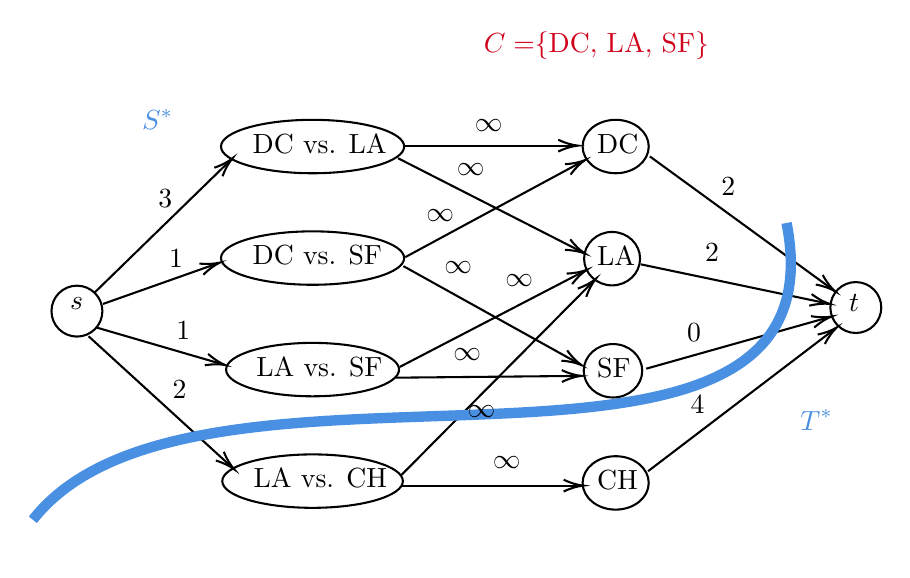
\begin{tikzpicture}[x=0.65pt,y=0.65pt,yscale=-1,xscale=1]
%uncomment if require: \path (0,459); %set diagram left start at 0, and has height of 459

%Straight Lines [id:da29828191190457176] 
\draw    (95,153) -- (170.57,79.4) ;
\draw [shift={(172,78)}, rotate = 135.75] [color={rgb, 255:red, 0; green, 0; blue, 0 }  ][line width=0.75]    (10.93,-3.29) .. controls (6.95,-1.4) and (3.31,-0.3) .. (0,0) .. controls (3.31,0.3) and (6.95,1.4) .. (10.93,3.29)   ;
%Straight Lines [id:da9886659900165116] 
\draw    (100,159) -- (163.11,136.67) ;
\draw [shift={(165,136)}, rotate = 160.51] [color={rgb, 255:red, 0; green, 0; blue, 0 }  ][line width=0.75]    (10.93,-3.29) .. controls (6.95,-1.4) and (3.31,-0.3) .. (0,0) .. controls (3.31,0.3) and (6.95,1.4) .. (10.93,3.29)   ;
%Straight Lines [id:da3998356428655834] 
\draw    (96,172) -- (166.08,192.44) ;
\draw [shift={(168,193)}, rotate = 196.26] [color={rgb, 255:red, 0; green, 0; blue, 0 }  ][line width=0.75]    (10.93,-3.29) .. controls (6.95,-1.4) and (3.31,-0.3) .. (0,0) .. controls (3.31,0.3) and (6.95,1.4) .. (10.93,3.29)   ;
%Straight Lines [id:da6630478389251291] 
\draw    (92,177) -- (171.52,249.65) ;
\draw [shift={(173,251)}, rotate = 222.41] [color={rgb, 255:red, 0; green, 0; blue, 0 }  ][line width=0.75]    (10.93,-3.29) .. controls (6.95,-1.4) and (3.31,-0.3) .. (0,0) .. controls (3.31,0.3) and (6.95,1.4) .. (10.93,3.29)   ;
%Straight Lines [id:da7357950429050455] 
\draw    (268,71) -- (362,71) ;
\draw [shift={(364,71)}, rotate = 180] [color={rgb, 255:red, 0; green, 0; blue, 0 }  ][line width=0.75]    (10.93,-3.29) .. controls (6.95,-1.4) and (3.31,-0.3) .. (0,0) .. controls (3.31,0.3) and (6.95,1.4) .. (10.93,3.29)   ;
%Straight Lines [id:da20538179275924828] 
\draw    (264,78) -- (366.22,130.09) ;
\draw [shift={(368,131)}, rotate = 207] [color={rgb, 255:red, 0; green, 0; blue, 0 }  ][line width=0.75]    (10.93,-3.29) .. controls (6.95,-1.4) and (3.31,-0.3) .. (0,0) .. controls (3.31,0.3) and (6.95,1.4) .. (10.93,3.29)   ;
%Straight Lines [id:da5590976987316391] 
\draw    (268,133) -- (366.24,79.95) ;
\draw [shift={(368,79)}, rotate = 151.63] [color={rgb, 255:red, 0; green, 0; blue, 0 }  ][line width=0.75]    (10.93,-3.29) .. controls (6.95,-1.4) and (3.31,-0.3) .. (0,0) .. controls (3.31,0.3) and (6.95,1.4) .. (10.93,3.29)   ;
%Straight Lines [id:da12638756166282472] 
\draw    (267,138) -- (364.25,192.03) ;
\draw [shift={(366,193)}, rotate = 209.05] [color={rgb, 255:red, 0; green, 0; blue, 0 }  ][line width=0.75]    (10.93,-3.29) .. controls (6.95,-1.4) and (3.31,-0.3) .. (0,0) .. controls (3.31,0.3) and (6.95,1.4) .. (10.93,3.29)   ;
%Straight Lines [id:da5033534492664359] 
\draw    (265,194) -- (367.23,140.92) ;
\draw [shift={(369,140)}, rotate = 152.56] [color={rgb, 255:red, 0; green, 0; blue, 0 }  ][line width=0.75]    (10.93,-3.29) .. controls (6.95,-1.4) and (3.31,-0.3) .. (0,0) .. controls (3.31,0.3) and (6.95,1.4) .. (10.93,3.29)   ;
%Straight Lines [id:da8320023848041241] 
\draw    (263,200) -- (364,199.02) ;
\draw [shift={(366,199)}, rotate = 179.44] [color={rgb, 255:red, 0; green, 0; blue, 0 }  ][line width=0.75]    (10.93,-3.29) .. controls (6.95,-1.4) and (3.31,-0.3) .. (0,0) .. controls (3.31,0.3) and (6.95,1.4) .. (10.93,3.29)   ;
%Straight Lines [id:da12872737382850508] 
\draw    (266,254) -- (372.59,146.42) ;
\draw [shift={(374,145)}, rotate = 134.74] [color={rgb, 255:red, 0; green, 0; blue, 0 }  ][line width=0.75]    (10.93,-3.29) .. controls (6.95,-1.4) and (3.31,-0.3) .. (0,0) .. controls (3.31,0.3) and (6.95,1.4) .. (10.93,3.29)   ;
%Straight Lines [id:da8484636178289252] 
\draw    (266,260) -- (365,260) ;
\draw [shift={(367,260)}, rotate = 180] [color={rgb, 255:red, 0; green, 0; blue, 0 }  ][line width=0.75]    (10.93,-3.29) .. controls (6.95,-1.4) and (3.31,-0.3) .. (0,0) .. controls (3.31,0.3) and (6.95,1.4) .. (10.93,3.29)   ;
%Straight Lines [id:da0981113218239027] 
\draw    (403,252) -- (506.41,173.21) ;
\draw [shift={(508,172)}, rotate = 142.7] [color={rgb, 255:red, 0; green, 0; blue, 0 }  ][line width=0.75]    (10.93,-3.29) .. controls (6.95,-1.4) and (3.31,-0.3) .. (0,0) .. controls (3.31,0.3) and (6.95,1.4) .. (10.93,3.29)   ;
%Straight Lines [id:da7431038981588827] 
\draw    (402,195) -- (503.07,166.54) ;
\draw [shift={(505,166)}, rotate = 164.28] [color={rgb, 255:red, 0; green, 0; blue, 0 }  ][line width=0.75]    (10.93,-3.29) .. controls (6.95,-1.4) and (3.31,-0.3) .. (0,0) .. controls (3.31,0.3) and (6.95,1.4) .. (10.93,3.29)   ;
%Straight Lines [id:da46241455607409654] 
\draw    (399,137) -- (502.04,158.59) ;
\draw [shift={(504,159)}, rotate = 191.83] [color={rgb, 255:red, 0; green, 0; blue, 0 }  ][line width=0.75]    (10.93,-3.29) .. controls (6.95,-1.4) and (3.31,-0.3) .. (0,0) .. controls (3.31,0.3) and (6.95,1.4) .. (10.93,3.29)   ;
%Straight Lines [id:da29204844875012814] 
\draw    (404,77) -- (505.38,150.82) ;
\draw [shift={(507,152)}, rotate = 216.06] [color={rgb, 255:red, 0; green, 0; blue, 0 }  ][line width=0.75]    (10.93,-3.29) .. controls (6.95,-1.4) and (3.31,-0.3) .. (0,0) .. controls (3.31,0.3) and (6.95,1.4) .. (10.93,3.29)   ;
%Curve Lines [id:da09781064377979187] 
\draw [color={rgb, 255:red, 74; green, 144; blue, 226 }  ,draw opacity=1 ][line width=3.75]    (61,279) .. controls (152,163) and (515,293) .. (480,114) ;

% Text Node
\draw    (216.5, 71.5) circle [x radius= 50.91, y radius= 14.85]   ;
\draw (181.5,63) node [anchor=north west][inner sep=0.75pt]   [align=left] {DC vs. LA};
% Text Node
\draw    (216.5, 133.5) circle [x radius= 50.91, y radius= 14.85]   ;
\draw (181.5,125) node [anchor=north west][inner sep=0.75pt]   [align=left] {DC vs. SF};
% Text Node
\draw    (216.5, 195.5) circle [x radius= 48.08, y radius= 14.85]   ;
\draw (183.5,187) node [anchor=north west][inner sep=0.75pt]   [align=left] {LA vs. SF};
% Text Node
\draw    (216.5, 257.5) circle [x radius= 50.2, y radius= 14.85]   ;
\draw (182,249) node [anchor=north west][inner sep=0.75pt]   [align=left] {LA vs. CH};
% Text Node
\draw    (85.5, 163) circle [x radius= 14.15, y radius= 14.15]   ;
\draw (80,154) node [anchor=north west][inner sep=0.75pt]   [align=left] {$\displaystyle s$};
% Text Node
\draw    (385, 71.5) circle [x radius= 18.38, y radius= 14.85]   ;
\draw (373,63) node [anchor=north west][inner sep=0.75pt]   [align=left] {DC};
% Text Node
\draw    (383, 133.83) circle [x radius= 15.56, y radius= 14.85]   ;
\draw (373,125.33) node [anchor=north west][inner sep=0.75pt]   [align=left] {LA};
% Text Node
\draw    (383.5, 196.16) circle [x radius= 16.26, y radius= 14.85]   ;
\draw (373,187.66) node [anchor=north west][inner sep=0.75pt]   [align=left] {SF};
% Text Node
\draw    (385, 258.5) circle [x radius= 18.38, y radius= 14.85]   ;
\draw (373,250) node [anchor=north west][inner sep=0.75pt]   [align=left] {CH};
% Text Node
\draw    (518.5, 161) circle [x radius= 14.15, y radius= 14.15]   ;
\draw (513,152) node [anchor=north west][inner sep=0.75pt]   [align=left] {$\displaystyle t$};
% Text Node
\draw (129,94) node [anchor=north west][inner sep=0.75pt]   [align=left] {3};
% Text Node
\draw (135,127) node [anchor=north west][inner sep=0.75pt]   [align=left] {1};
% Text Node
\draw (139,167) node [anchor=north west][inner sep=0.75pt]   [align=left] {1};
% Text Node
\draw (137,200) node [anchor=north west][inner sep=0.75pt]   [align=left] {2};
% Text Node
\draw (442,87) node [anchor=north west][inner sep=0.75pt]   [align=left] {2};
% Text Node
\draw (433,124) node [anchor=north west][inner sep=0.75pt]   [align=left] {2};
% Text Node
\draw (423,168) node [anchor=north west][inner sep=0.75pt]   [align=left] {0};
% Text Node
\draw (425,208) node [anchor=north west][inner sep=0.75pt]   [align=left] {4};
% Text Node
\draw (305,55) node [anchor=north west][inner sep=0.75pt]   [align=left] {$\displaystyle \infty $};
% Text Node
\draw (295,79) node [anchor=north west][inner sep=0.75pt]   [align=left] {$\displaystyle \infty $};
% Text Node
\draw (278,105) node [anchor=north west][inner sep=0.75pt]   [align=left] {$\displaystyle \infty $};
% Text Node
\draw (288,134) node [anchor=north west][inner sep=0.75pt]   [align=left] {$\displaystyle \infty $};
% Text Node
\draw (322,141) node [anchor=north west][inner sep=0.75pt]   [align=left] {$\displaystyle \infty $};
% Text Node
\draw (293,182) node [anchor=north west][inner sep=0.75pt]   [align=left] {$\displaystyle \infty $};
% Text Node
\draw (301,214) node [anchor=north west][inner sep=0.75pt]   [align=left] {$\displaystyle \infty $};
% Text Node
\draw (315,242) node [anchor=north west][inner sep=0.75pt]   [align=left] {$\displaystyle \infty $};
% Text Node
\draw (310,6) node [anchor=north west][inner sep=0.75pt]  [color={rgb, 255:red, 208; green, 2; blue, 27 }  ,opacity=1 ] [align=left] {$\displaystyle C=$\{DC, LA, SF\}};
% Text Node
\draw (486,216) node [anchor=north west][inner sep=0.75pt]  [color={rgb, 255:red, 74; green, 144; blue, 226 }  ,opacity=1 ] [align=left] {$\displaystyle \textcolor[rgb]{0.29,0.56,0.89}{T^{*}}$};
% Text Node
\draw (120,49) node [anchor=north west][inner sep=0.75pt]  [color={rgb, 255:red, 74; green, 144; blue, 226 }  ,opacity=1 ] [align=left] {$\displaystyle \textcolor[rgb]{0.29,0.56,0.89}{S^{*}}$};


\end{tikzpicture}

